\chapter{Elektronik}\label{anh:kap:elektronik}

\section{Elektronik der
Signalgenerierung}\label{anh:sec:signalgenerierung_elektronik} In diesem
Abschnitt soll die Elektronik der Signalgenerierung, die in Abschn. \ref{subsec:signalgenerierung} erwähnt wurde, genauer betrachtet werden.
Ziel ist es, aus dem Fringepattern-Signal des FPIs digital lesbare Signale zu
generieren, mit denen man die Zeit zwischen Beginn der
Spannungsrampe und Offsetfringe bzw. zwischen Offsetfringe
und Interfringe messen kann. Exemplarisch wird die Signalgenerierung hier
für einen Laser erklärt. Selbstverständlich besteht der komplette
Schaltkreis aus vier identischen Kopien der in Abb.
\ref{fig:signalgenerierung_schaltplan} dargestellten Schaltung.\par
\begin{figure}[h]
 	\centering
 	\fbox{\parbox{\dimexpr \linewidth - 2\fboxrule - 2\fboxsep}{
		\subfloat[]{
			\label{subfig:signalgenerierung_schaltplan_01}
	    	\includegraphics[width=(\textwidth-1cm)]{gfx/signalgenerierung_schaltplan_01}
	    }\\
		\subfloat[]{
			\label{subfig:signalgenerierung_schaltplan_02}
	    	\includegraphics[width=(\textwidth-1cm)]{gfx/signalgenerierung_schaltplan_02}
	    }\\
	    \subfloat[]{
			\label{subfig:signalgenerierung_schaltplan_03}
	    	\includegraphics[width=(\textwidth-1cm)]{gfx/signalgenerierung_schaltplan_03}
	    }
	}}
	\caption[Signalgenerierung - Schaltplan]{Schaltplan der
	Signalgenerierung zum
	Fringe-Offset-Locking (aus
	\cite{signalgenerierung})}\label{fig:signalgenerierung_schaltplan}
\end{figure}
Um elektronisch ein Fringemaximum zu detektieren ist es nötig die Ableitung
des Signals zu generieren. Abbildung
\ref{subfig:signalgenerierung_schaltplan_01} zeigt den ersten Teil der Schaltung. Über den rückgekoppelten Operationsverstärker
\textit{TL082} wird die Ableitung gebildet und somit ein Signal an (7)
erzeugt, das einen steilen Nulldurchgang mit negativer Steigung bei jedem Fringe hat und über einen
Monitor-Ausgang (DIF0) betrachtet werden kann. Danach wird ein
hysteretischer Komparator \textit{AD790} verwendet, der oberhalb eines
bestimmten Spannungsniveaus ein digitales HIGH und unterhalb eines bestimmten Spannungsniveaus
ein digitales LOW an (7) ausgibt. Der Zwischenzustand von (7) ist
davon abhängig, ob die Spannung von unterhalb des unteren Niveaus oder von
oberhalb des oberen Niveaus kommt. Somit schaltet der Komparator kurz vor dem
Maximum des Fringes auf HIGH und bei unterem Niveau von $0\,$V genau am
Nulldurchgang der Ableitung, also am Maximum des Fringes, auf LOW. Die
Teilschaltung mit dem IC \textit{74LS123} reagiert auf die fallende Flanke des
TTL-Pulses des Komparators und erzeugt beginnend am
Nulldurchgang der Ableitung selbst einen kurzen TTL-Puls (T1) mit einer
Länge, die von der Wahl des vorgeschalteten Widerstandes und des
Kondensators abhängt.\par Das Gate des Rampengenerators ((STARTTTL) in Abb.
\ref{subfig:signalgenerierung_schaltplan_02}) ist bei fallender Spannungsrampe
HIGH und bei steigender Spannungsrampe LOW. Im ersten Teil der Schaltung
\ref{subfig:signalgenerierung_schaltplan_02} bewirkt dies einen durch das
Drehpotentiometer in der Länge einstellbaren TTL-Puls am Anfang der steigenden
Spannungsrampe. Das Ende der steigenden Spannungsrampe wird ignoriert.
Mit einer Zeitverzögerung von der Länge des erzeugten TTL-Pulses wird dann im
zweiten Teil der Schaltung \ref{subfig:signalgenerierung_schaltplan_02} ein weiterer TTL-Puls erzeugt.
Dadurch wird eine Verzögerung des Starttriggers der steigenden Rampe bewirkt, um
den Start der Fringe-Detektion zu verschieben und so die zu Beginn der Rampe
auftretende Nichtlinearität zu ignorieren.\par
Schaltung \ref{subfig:signalgenerierung_schaltplan_03} ist nun für die Erzeugung
der in \ref{fig:FPI_signal-zeitverlauf}(d,e) dargestellten TTL-Pulse zuständig. Sie
besteht aus zwei NOR-Flipflops (links und rechts) und wiederum aus dem IC
\textit{74LS123} in der Mitte, welcher nun sensitiv auf eine steigende
Pulsflanke ist. Im Ausgangszustand liegt an den beiden Eingängen und am unteren
Ausgang des linken Flipflops LOW an. Der verzögerte kurze Start-TTL-Puls kommt
nun am Set-Eingang des linken Flipflops (CLK1) an und setzt den unteren
Ausgang, der den Offsetfringe-TTL-Puls durch (CLKB1) repräsentiert, auf HIGH.
Der Counter für die Offsetfringezeit beginnt zu zählen. Der Offsetfringe
erzeugt nun an (T1) einen kurzen TTL-Puls, welcher den linken Flipflop zurücksetzt. (CLKB1) wird also LOW und der Counter
für die die Offsetfringezeit stoppt. Der obere Ausgang des ersten Flipflops
wechselt somit auf HIGH, was einen kurzen TTL-Puls am Ausgang Q von
\textit{74LS123} auslöst. Dadurch wird der Ausgang des rechten FlipFlops (CLKA1) auf HIGH gesetzt
und der Counter für die Interfringezeit beginnt zu zählen. Damit durch den
kurzen Puls an (T1) nicht der verbotene Eingangszustand HIGH/HIGH am rechten
Flipflop anliegt, wird dieser durch ein effektives AND mit
$\overline{\text{Q}}$, das zu diesem Zeitpunkt kurz LOW ist, verknüpft. Der
Interfringe löst wieder einen TTL Puls an (T1) aus und setzt nun den rechten
Flipflop zurück, was auch den Counter für die Interfringezeit stoppt.\par
Mit dieser Schaltung können also die Transmissionssignale des FPIs in digitale
Signale für die Counterkarte umgesetzt werden.

\section{Counterkarte}\label{anh:sec:counterkarte}
In diesem Abschnitt soll detailliert auf die Elektronik der Counterkarte
eingegangen werden. An sie werden die TTL-Signale der in Abschn.
\ref{anh:kap:signalgenerierung_elektronik} erklärten Signalgenerierung für das
Fringepattern weitergeleitet, mit denen sie die Offsetfringe- und
Interfringezeiten eines Diodenlasers und des Referenzlasers messen kann.
Abbildung \ref{fig:counterkarte_schaltplan} zeigt den Schaltplan der
Counterkarte. Die Platine ist noch einmal in Abb.
\ref{fig:counterkarte_foto} als Foto abgebildet.\par
\begin{figure}[h]
 	\centering
 	\fbox{\parbox{\dimexpr \linewidth - 2\fboxrule - 2\fboxsep}{
 	\centering
	    \includegraphics[width=\textwidth-2cm]{gfx/counterkarte_foto}
	    }}
	\caption[Counterkarte -
	Foto]{Foto der Counterkarte}\label{fig:counterkarte_foto}
\end{figure}
Das Gate des Rampengenerators wird an der Lemobuchse (X10) abgegriffen.
Über den Jumper \textit{JP3} lässt sich das Rohsignal oder die Invertierung weiterverwenden.
Hier ist eine Invertierung nötig, womit die steigende Spannungsrampe einem HIGH entspricht.
Über das AND \textit{IC20} ist somit der Taktgeber \textit{IC17} bei steigender
Rampe aktiviert. Die Taktrate ist über \textit{JP4} einstellbar. Der Bereich
\textit{Clear Counter \& D-FF Manuell/Arduino/Atmega} erzeugt aus der
steigenden Flanke des Gates (also aus dem Übergang von fallender zu steigender
Rampe) einen verzögerten $1\,$\textmu s langen Puls, mit dem die vier Counter
des Typs \textit{SN74LV8154PW} zurückgesetzt werden, sofern Jumper \textit{JP2}
gesetzt ist. Gleichzeitig werden auch die getakteten Flipflops \textit{IC6A/B}
und \textit{IC15A/B}, deren Ausgänge die Status-Bits darstellen, zurückgesetzt.
Andernfalls müssen die Counter vor jeder Rampe üer die Anschlüsse
($\overline{\text{CLR}}$) oder ($\overline{\text{CLR2}}$) zurückgesetzt werden.
Über die Lemobuchsen (X1), (X7), (X8) und (X9) erhält die Karte die TTL-Signale
der Signalgenerierung. Ist eines dieser TTL-Signale HIGH, zählt der
entsprechende Counter mit der vorgegebenen Taktrate hoch. Beim Eintreten des
entsprechenden Fringes, also bei fallender Flanke, wird über einen der Bausteine
\textit{IC5A/B} und \textit{IC14A/B} ein kurzer TTL-Puls ausgelöst, der den
Counterwerte in die Counterregister schiebt. Gleichzeitig wird über das
entsprechende Flipflop das Status-Bit gesetzt.\par
Über die Anschlüsse (DORR), (DIRR), (DODR) und (DIDR) können die Status-Bits
ausgelesen werden. Die verschiedenen Counterregister können über (Addr. 0),
(Addr. 1) und (Addr. 2) adressiert werden. Tabelle
\ref{tab:adressbus_kodierung} schlüsselt die Adresskodierung auf. Um die
Adressierung zu aktivieren muss (Enable) auf HIGH gesetzt werden. An (Y0) bis (Y7) liegt dann das Byte des entsprechenden Registers an.\par
Als Erweiterung wurde auf dieselbe Platine das Interface für einen modularen
unabhängigen vierfachen 16-Bit DAC implementiert, der die Modulation von
Laserparametern übernehmen könnte. Somit ist es möglich die Counterkarte auch in Systemen einzusetzen, in
denen ausschließlich über FOL wird. Ein
zwischengeschalteter Mikrocontroller würde die Regelung übernehmen. Details über
den DAC können \cite{counterkarte_laserstabilisierung} entnommen werden.
\begin{landscape}
	\begin{figure}
	 	\centering
	 	\fbox{\parbox{\dimexpr \linewidth - 2\fboxrule - 2\fboxsep}{
	 	\centering
		    \includegraphics[height=\textwidth-0cm]{gfx/counterkarte_schaltplan}
		    }}
		\caption[Counterkarte -
		Schaltplan]{Schaltplan der Counterkarte (aus \cite{counterkarte_laserstabilisierung})}\label{fig:counterkarte_schaltplan}
	\end{figure}
\end{landscape}

\chapter{Software}\label{anh:kap:software}

\section{Quelltext
Datenaufbereitung}\label{anh:kap:quelltext_arduino_laserinformationsverarbeitung} Im Folgenden ist der Quelltext des Programms für den Mikrocontroller
\textit{Arduino} zur Datenaufbereitung der Laserinformationen abgedruckt. Das
Programm wurde in einer an den Arduino angepassten Version der
Programmiersprache C geschrieben. Alle Kommentare sind in englisch gehalten.
\lstinputlisting[]{code/arduino_laserinformation.c}

\section{Quelltext
Countratenauslese}\label{anh:sec:quelltext_arduino_countrate} Im Folgenden kann
der Quelltext des Programms für den Arduino zur Countratenauslese aus der Counterkarte für die Countraten eingesehen werden. Die
Kommunikation mit der Counterkarte erfolgt über eine SPI-Schnittstelle. Die
Daten werden anschließend an den PC via RS232 weitergeleitet.
\lstinputlisting[]{code/arduino_countrate.c}

\chapter{Charakterisierung des Systems}\label{anh:kap:charakterisierung}

\section{Simulationen Nonius-Methode}\label{anh:sec:nonius_simulationen}
In diesem Abschnitt werden die Simulationen für die FSR-Bestimmung des FPIs
vorgestellt. Es folgt der \textit{Mathematica}-Quelltext für die Simulation:
\lstset{language=Mathematica}
\lstinputlisting[]{code/nonius_simulation.txt}
Abbildung \ref{fig:nonius_FSR_simulation} zeigt die Simulation für verschiedene
$a$ und $7$ Relativfrequenzen. Angenommen wurde ein FSR von $300\,$MHz. Die
Wavemetergenauigkeit wurde auf $40\,$MHz festegelegt und die simulierten
Frequenzen entsprechend zufällig variiert.
\begin{figure}[H]
 	\centering
 	\fbox{\parbox{\dimexpr \linewidth - 2\fboxrule - 2\fboxsep}{
 	\subfloat[]{
		\label{subfig:nonius_FSR_simulation_a2}
		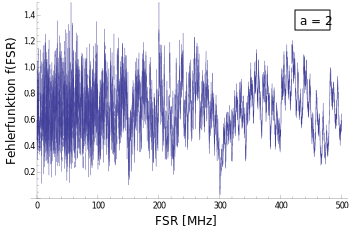
\includegraphics[width=(\textwidth-0.6cm)/2]{plt/nonius_FSR_simulation_a2}
		}
 	\subfloat[]{
		\label{subfig:nonius_FSR_simulation_a3}
		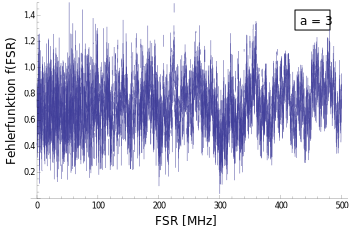
\includegraphics[width=(\textwidth-0.6cm)/2]{plt/nonius_FSR_simulation_a3}
		}\\
	 \subfloat[]{
		\label{subfig:nonius_FSR_simulation_a4}
		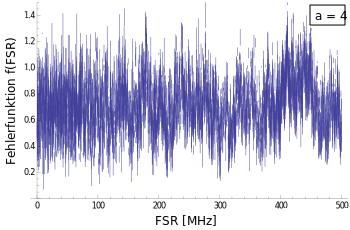
\includegraphics[width=(\textwidth-0.6cm)/2]{plt/nonius_FSR_simulation_a4}
		}
	\subfloat[]{
		\label{subfig:nonius_FSR_simulation_a5}
		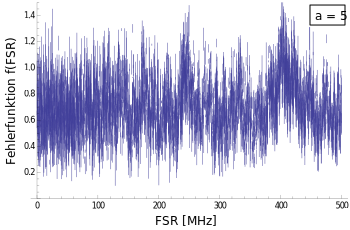
\includegraphics[width=(\textwidth-0.6cm)/2]{plt/nonius_FSR_simulation_a5}
		}
	}}
	\caption[Simulationen Nonius-Methode]{Die Abbildung zeigt Plots der
	Simulationen zur Bestimmung des FSR mit verscheidenen $a$ und $7$ Relativfrequnenzen.}
	\label{fig:nonius_FSR_simulation}
\end{figure}
\section{Laserstabilität}\label{anh:sec:laserstabilitaet}
In diesem Abschnitt finden sich die Plots des Frequenzverhaltens eines jeden
Lasers im neuen System und des Lasers für den zweiten Anregungsschitts im alten
System. Es wird unterschieden zwischen freilaufend, \textit{iScan}-stabilisiert
und \textit{iScan}+FOL-stabilisiert.
\begin{figure}[hp]
 	\centering
 	\footnotesize
 	\fbox{\parbox{\dimexpr \linewidth - 2\fboxrule - 2\fboxsep}{
 	\subfloat[]{
		\label{subfig:laserstabilitaet_a_freilaufend}
		\input{plt/laserstabilitaet_a_freilaufend}
		}\\
 	\subfloat[]{
		\label{subfig:laserstabilitaet_a_iScan}
		\input{plt/laserstabilitaet_a_iScan}
		}\\
	 \subfloat[]{
		\label{subfig:laserstabilitaet_a_iScan+FOL}
		% GNUPLOT: LaTeX picture with Postscript
\begingroup
  \makeatletter
  \providecommand\color[2][]{%
    \GenericError{(gnuplot) \space\space\space\@spaces}{%
      Package color not loaded in conjunction with
      terminal option `colourtext'%
    }{See the gnuplot documentation for explanation.%
    }{Either use 'blacktext' in gnuplot or load the package
      color.sty in LaTeX.}%
    \renewcommand\color[2][]{}%
  }%
  \providecommand\includegraphics[2][]{%
    \GenericError{(gnuplot) \space\space\space\@spaces}{%
      Package graphicx or graphics not loaded%
    }{See the gnuplot documentation for explanation.%
    }{The gnuplot epslatex terminal needs graphicx.sty or graphics.sty.}%
    \renewcommand\includegraphics[2][]{}%
  }%
  \providecommand\rotatebox[2]{#2}%
  \@ifundefined{ifGPcolor}{%
    \newif\ifGPcolor
    \GPcolortrue
  }{}%
  \@ifundefined{ifGPblacktext}{%
    \newif\ifGPblacktext
    \GPblacktexttrue
  }{}%
  % define a \g@addto@macro without @ in the name:
  \let\gplgaddtomacro\g@addto@macro
  % define empty templates for all commands taking text:
  \gdef\gplbacktext{}%
  \gdef\gplfronttext{}%
  \makeatother
  \ifGPblacktext
    % no textcolor at all
    \def\colorrgb#1{}%
    \def\colorgray#1{}%
  \else
    % gray or color?
    \ifGPcolor
      \def\colorrgb#1{\color[rgb]{#1}}%
      \def\colorgray#1{\color[gray]{#1}}%
      \expandafter\def\csname LTw\endcsname{\color{white}}%
      \expandafter\def\csname LTb\endcsname{\color{black}}%
      \expandafter\def\csname LTa\endcsname{\color{black}}%
      \expandafter\def\csname LT0\endcsname{\color[rgb]{1,0,0}}%
      \expandafter\def\csname LT1\endcsname{\color[rgb]{0,1,0}}%
      \expandafter\def\csname LT2\endcsname{\color[rgb]{0,0,1}}%
      \expandafter\def\csname LT3\endcsname{\color[rgb]{1,0,1}}%
      \expandafter\def\csname LT4\endcsname{\color[rgb]{0,1,1}}%
      \expandafter\def\csname LT5\endcsname{\color[rgb]{1,1,0}}%
      \expandafter\def\csname LT6\endcsname{\color[rgb]{0,0,0}}%
      \expandafter\def\csname LT7\endcsname{\color[rgb]{1,0.3,0}}%
      \expandafter\def\csname LT8\endcsname{\color[rgb]{0.5,0.5,0.5}}%
    \else
      % gray
      \def\colorrgb#1{\color{black}}%
      \def\colorgray#1{\color[gray]{#1}}%
      \expandafter\def\csname LTw\endcsname{\color{white}}%
      \expandafter\def\csname LTb\endcsname{\color{black}}%
      \expandafter\def\csname LTa\endcsname{\color{black}}%
      \expandafter\def\csname LT0\endcsname{\color{black}}%
      \expandafter\def\csname LT1\endcsname{\color{black}}%
      \expandafter\def\csname LT2\endcsname{\color{black}}%
      \expandafter\def\csname LT3\endcsname{\color{black}}%
      \expandafter\def\csname LT4\endcsname{\color{black}}%
      \expandafter\def\csname LT5\endcsname{\color{black}}%
      \expandafter\def\csname LT6\endcsname{\color{black}}%
      \expandafter\def\csname LT7\endcsname{\color{black}}%
      \expandafter\def\csname LT8\endcsname{\color{black}}%
    \fi
  \fi
  \setlength{\unitlength}{0.0500bp}%
  \begin{picture}(7936.00,3968.00)%
    \gplgaddtomacro\gplbacktext{%
      \csname LTb\endcsname%
      \put(1080,1587){\makebox(0,0)[r]{\strut{}-20}}%
      \put(1080,1847){\makebox(0,0)[r]{\strut{}-15}}%
      \put(1080,2107){\makebox(0,0)[r]{\strut{}-10}}%
      \put(1080,2367){\makebox(0,0)[r]{\strut{}-5}}%
      \put(1080,2627){\makebox(0,0)[r]{\strut{} 0}}%
      \put(1080,2887){\makebox(0,0)[r]{\strut{} 5}}%
      \put(1080,3147){\makebox(0,0)[r]{\strut{} 10}}%
      \put(1080,3407){\makebox(0,0)[r]{\strut{} 15}}%
      \put(1080,3667){\makebox(0,0)[r]{\strut{} 20}}%
      \put(1080,3927){\makebox(0,0)[r]{\strut{} 25}}%
      \put(1200,1387){\makebox(0,0){\strut{}}}%
      \put(2263,1387){\makebox(0,0){\strut{}}}%
      \put(3325,1387){\makebox(0,0){\strut{}}}%
      \put(4388,1387){\makebox(0,0){\strut{}}}%
      \put(5450,1387){\makebox(0,0){\strut{}}}%
      \put(6513,1387){\makebox(0,0){\strut{}}}%
      \put(7575,1387){\makebox(0,0){\strut{}}}%
      \put(380,2957){\rotatebox{-270}{\makebox(0,0){\strut{}relative Frequenz [MHz]}}}%
    }%
    \gplgaddtomacro\gplfronttext{%
    }%
    \gplgaddtomacro\gplbacktext{%
      \csname LTb\endcsname%
      \put(1080,647){\makebox(0,0)[r]{\strut{} 5}}%
      \put(1080,894){\makebox(0,0)[r]{\strut{} 10}}%
      \put(1080,1140){\makebox(0,0)[r]{\strut{} 15}}%
      \put(1200,200){\makebox(0,0){\strut{}0}}%
      \put(2263,200){\makebox(0,0){\strut{}20}}%
      \put(3325,200){\makebox(0,0){\strut{}40}}%
      \put(4388,200){\makebox(0,0){\strut{}60}}%
      \put(5450,200){\makebox(0,0){\strut{}80}}%
      \put(6513,200){\makebox(0,0){\strut{}100}}%
      \put(7575,200){\makebox(0,0){\strut{}120}}%
      \put(380,893){\rotatebox{-270}{\makebox(0,0){\strut{}Jitter [MHz]}}}%
      \put(4387,0){\makebox(0,0){\strut{}Zeit [min]}}%
    }%
    \gplgaddtomacro\gplfronttext{%
    }%
    \gplbacktext
    \put(0,0){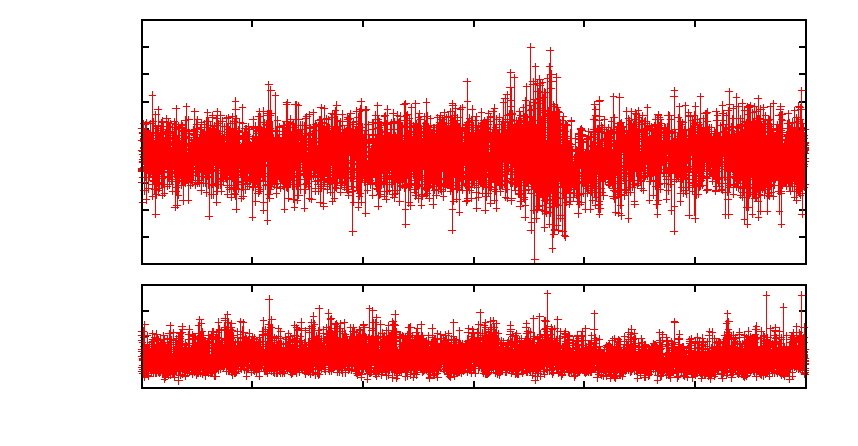
\includegraphics{laserstabilitaet_a_iScan+FOL}}%
    \gplfronttext
  \end{picture}%
\endgroup

		}
	}}
	\caption[Laserfrequenzverhalten blauer Laser]{Die Abbildung zeigt das
	Laserfrequenzverhalten des blauen Lasers im freilaufenden (a),
	\textit{iScan}-stabiliserten (b) und \textit{iScan}+FOL-stabiliserten Modus
	(c). Unten ist jeweils der Jitter aufgetragen.}
	\label{fig:laserstabilitaet_a}
\end{figure}
\begin{figure}[hp]
 	\centering
 	\footnotesize
 	\fbox{\parbox{\dimexpr \linewidth - 2\fboxrule - 2\fboxsep}{
 	\subfloat[]{
		\label{subfig:laserstabilitaet_b_freilaufend}
		\input{plt/laserstabilitaet_b_freilaufend}
		}\\
 	\subfloat[]{
		\label{subfig:laserstabilitaet_b_iScan}
		\input{plt/laserstabilitaet_b_iScan}
		}\\
	 \subfloat[]{
		\label{subfig:laserstabilitaet_b_iScan+FOL}
		\input{plt/laserstabilitaet_b_iScan+FOL}
		}
	}}
	\caption[Laserfrequenzverhalten \textit{DL-Pro}]{Die Abbildung zeigt das
	Laserfrequenzverhalten des \textit{DL-Pro} im freilaufenden (a),
	\textit{iScan}-stabiliserten (b) und \textit{iScan}+FOL-stabiliserten Modus
	(c). Unten ist jeweils der Jitter aufgetragen.}
	\label{fig:laserstabilitaet_b}
\end{figure}
\begin{figure}[hp]
 	\centering
 	\footnotesize
 	\fbox{\parbox{\dimexpr \linewidth - 2\fboxrule - 2\fboxsep}{
 	\subfloat[]{
		\label{subfig:laserstabilitaet_c_freilaufend}
		\input{plt/laserstabilitaet_c_freilaufend}
		}\\
 	\subfloat[]{
		\label{subfig:laserstabilitaet_c_iScan}
		\input{plt/laserstabilitaet_c_iScan}
		}\\
	 \subfloat[]{
		\label{subfig:laserstabilitaet_c_iScan+FOL}
		\input{plt/laserstabilitaet_c_iScan+FOL}
		}
	}}
	\caption[Laserfrequenzverhalten \textit{TA-Pro}]{Die Abbildung zeigt das
	Laserfrequenzverhalten des \textit{TA-Pro} im freilaufenden (a),
	\textit{iScan}-stabiliserten (b) und \textit{iScan}+FOL-stabiliserten Modus
	(c). Unten ist jeweils der Jitter aufgetragen.}
	\label{fig:laserstabilitaet_c}
\end{figure}
\begin{figure}[hp]
 	\centering
 	\footnotesize
 	\fbox{\parbox{\dimexpr \linewidth - 2\fboxrule - 2\fboxsep}{
 	\subfloat[]{
		\label{subfig:laserstabilitaet_alt_freilaufend}
		\input{plt/laserstabilitaet_alt_freilaufend}
		}\\
	 \subfloat[]{
		\label{subfig:laserstabilitaet_alt_FOL}
		\input{plt/laserstabilitaet_alt_FOL}
		}
	}}
	\caption[Laserfrequenzverhalten \textit{TA-Pro}]{Die Abbildung zeigt das
	Laserfrequenzverhalten des Lasers für den zweiten Anregungsschritt aus dem
	alten System im freilaufenden (a) und FOL-stabiliserten Modus (c). Unten ist
	jeweils der Jitter aufgetragen.}
	\label{fig:laserstabilitaet_c}
\end{figure}

\newpage
\section{Linearisierung der
\textit{iScans}}\label{anh:sec:linearisierung}
In Abb. \ref{fig:linearisierung_FSR_korr_anh} werden die einzelnen
Fringepatternanalysen für die Datenpunkte der Plots in Abb.
\ref{fig:linearisierung_FSR_korr} gezeigt.
\begin{figure}[hb]
 	\centering
 	\footnotesize
 	\fbox{\parbox{\dimexpr \linewidth - 2\fboxrule - 2\fboxsep}{
 	\subfloat[Messung 1 / Korrektur 1]{
		\label{subfig:linearisierung_FSR_korr_anh_01}
		% GNUPLOT: LaTeX picture with Postscript
\begingroup
  \makeatletter
  \providecommand\color[2][]{%
    \GenericError{(gnuplot) \space\space\space\@spaces}{%
      Package color not loaded in conjunction with
      terminal option `colourtext'%
    }{See the gnuplot documentation for explanation.%
    }{Either use 'blacktext' in gnuplot or load the package
      color.sty in LaTeX.}%
    \renewcommand\color[2][]{}%
  }%
  \providecommand\includegraphics[2][]{%
    \GenericError{(gnuplot) \space\space\space\@spaces}{%
      Package graphicx or graphics not loaded%
    }{See the gnuplot documentation for explanation.%
    }{The gnuplot epslatex terminal needs graphicx.sty or graphics.sty.}%
    \renewcommand\includegraphics[2][]{}%
  }%
  \providecommand\rotatebox[2]{#2}%
  \@ifundefined{ifGPcolor}{%
    \newif\ifGPcolor
    \GPcolortrue
  }{}%
  \@ifundefined{ifGPblacktext}{%
    \newif\ifGPblacktext
    \GPblacktexttrue
  }{}%
  % define a \g@addto@macro without @ in the name:
  \let\gplgaddtomacro\g@addto@macro
  % define empty templates for all commands taking text:
  \gdef\gplbacktext{}%
  \gdef\gplfronttext{}%
  \makeatother
  \ifGPblacktext
    % no textcolor at all
    \def\colorrgb#1{}%
    \def\colorgray#1{}%
  \else
    % gray or color?
    \ifGPcolor
      \def\colorrgb#1{\color[rgb]{#1}}%
      \def\colorgray#1{\color[gray]{#1}}%
      \expandafter\def\csname LTw\endcsname{\color{white}}%
      \expandafter\def\csname LTb\endcsname{\color{black}}%
      \expandafter\def\csname LTa\endcsname{\color{black}}%
      \expandafter\def\csname LT0\endcsname{\color[rgb]{1,0,0}}%
      \expandafter\def\csname LT1\endcsname{\color[rgb]{0,1,0}}%
      \expandafter\def\csname LT2\endcsname{\color[rgb]{0,0,1}}%
      \expandafter\def\csname LT3\endcsname{\color[rgb]{1,0,1}}%
      \expandafter\def\csname LT4\endcsname{\color[rgb]{0,1,1}}%
      \expandafter\def\csname LT5\endcsname{\color[rgb]{1,1,0}}%
      \expandafter\def\csname LT6\endcsname{\color[rgb]{0,0,0}}%
      \expandafter\def\csname LT7\endcsname{\color[rgb]{1,0.3,0}}%
      \expandafter\def\csname LT8\endcsname{\color[rgb]{0.5,0.5,0.5}}%
    \else
      % gray
      \def\colorrgb#1{\color{black}}%
      \def\colorgray#1{\color[gray]{#1}}%
      \expandafter\def\csname LTw\endcsname{\color{white}}%
      \expandafter\def\csname LTb\endcsname{\color{black}}%
      \expandafter\def\csname LTa\endcsname{\color{black}}%
      \expandafter\def\csname LT0\endcsname{\color{black}}%
      \expandafter\def\csname LT1\endcsname{\color{black}}%
      \expandafter\def\csname LT2\endcsname{\color{black}}%
      \expandafter\def\csname LT3\endcsname{\color{black}}%
      \expandafter\def\csname LT4\endcsname{\color{black}}%
      \expandafter\def\csname LT5\endcsname{\color{black}}%
      \expandafter\def\csname LT6\endcsname{\color{black}}%
      \expandafter\def\csname LT7\endcsname{\color{black}}%
      \expandafter\def\csname LT8\endcsname{\color{black}}%
    \fi
  \fi
  \setlength{\unitlength}{0.0500bp}%
  \begin{picture}(3968.00,2664.00)%
    \gplgaddtomacro\gplbacktext{%
      \csname LTb\endcsname%
      \put(740,540){\makebox(0,0)[r]{\strut{}-50}}%
      \csname LTb\endcsname%
      \put(740,890){\makebox(0,0)[r]{\strut{} 0}}%
      \csname LTb\endcsname%
      \put(740,1241){\makebox(0,0)[r]{\strut{} 50}}%
      \csname LTb\endcsname%
      \put(740,1591){\makebox(0,0)[r]{\strut{} 100}}%
      \csname LTb\endcsname%
      \put(740,1942){\makebox(0,0)[r]{\strut{} 150}}%
      \csname LTb\endcsname%
      \put(740,2292){\makebox(0,0)[r]{\strut{} 200}}%
      \csname LTb\endcsname%
      \put(740,2643){\makebox(0,0)[r]{\strut{} 250}}%
      \put(860,340){\makebox(0,0){\strut{}-1}}%
      \put(1135,340){\makebox(0,0){\strut{} 0}}%
      \put(1409,340){\makebox(0,0){\strut{} 1}}%
      \put(1684,340){\makebox(0,0){\strut{} 2}}%
      \put(1959,340){\makebox(0,0){\strut{} 3}}%
      \put(2233,340){\makebox(0,0){\strut{} 4}}%
      \put(2508,340){\makebox(0,0){\strut{} 5}}%
      \put(2783,340){\makebox(0,0){\strut{} 6}}%
      \put(3058,340){\makebox(0,0){\strut{} 7}}%
      \put(3332,340){\makebox(0,0){\strut{} 8}}%
      \put(3607,340){\makebox(0,0){\strut{} 9}}%
      \put(160,1591){\rotatebox{-270}{\makebox(0,0){\strut{}Abweichung [MHz]}}}%
      \put(2233,140){\makebox(0,0){\strut{}Scan Position [GHz]}}%
    }%
    \gplgaddtomacro\gplfronttext{%
      \csname LTb\endcsname%
      \put(2824,1842){\makebox(0,0)[r]{\strut{}\tiny{zw. Fringes [MHz]}}}%
      \csname LTb\endcsname%
      \put(2824,1642){\makebox(0,0)[r]{\strut{}\tiny{absolut [MHz]}}}%
    }%
    \gplbacktext
    \put(0,0){\includegraphics{linearisierung_FSR_korr/01}}%
    \gplfronttext
  \end{picture}%
\endgroup

	}
 	\subfloat[Messung 2 / Korrektur 2]{
		\label{subfig:linearisierung_FSR_korr_anh_02}
		% GNUPLOT: LaTeX picture with Postscript
\begingroup
  \makeatletter
  \providecommand\color[2][]{%
    \GenericError{(gnuplot) \space\space\space\@spaces}{%
      Package color not loaded in conjunction with
      terminal option `colourtext'%
    }{See the gnuplot documentation for explanation.%
    }{Either use 'blacktext' in gnuplot or load the package
      color.sty in LaTeX.}%
    \renewcommand\color[2][]{}%
  }%
  \providecommand\includegraphics[2][]{%
    \GenericError{(gnuplot) \space\space\space\@spaces}{%
      Package graphicx or graphics not loaded%
    }{See the gnuplot documentation for explanation.%
    }{The gnuplot epslatex terminal needs graphicx.sty or graphics.sty.}%
    \renewcommand\includegraphics[2][]{}%
  }%
  \providecommand\rotatebox[2]{#2}%
  \@ifundefined{ifGPcolor}{%
    \newif\ifGPcolor
    \GPcolortrue
  }{}%
  \@ifundefined{ifGPblacktext}{%
    \newif\ifGPblacktext
    \GPblacktexttrue
  }{}%
  % define a \g@addto@macro without @ in the name:
  \let\gplgaddtomacro\g@addto@macro
  % define empty templates for all commands taking text:
  \gdef\gplbacktext{}%
  \gdef\gplfronttext{}%
  \makeatother
  \ifGPblacktext
    % no textcolor at all
    \def\colorrgb#1{}%
    \def\colorgray#1{}%
  \else
    % gray or color?
    \ifGPcolor
      \def\colorrgb#1{\color[rgb]{#1}}%
      \def\colorgray#1{\color[gray]{#1}}%
      \expandafter\def\csname LTw\endcsname{\color{white}}%
      \expandafter\def\csname LTb\endcsname{\color{black}}%
      \expandafter\def\csname LTa\endcsname{\color{black}}%
      \expandafter\def\csname LT0\endcsname{\color[rgb]{1,0,0}}%
      \expandafter\def\csname LT1\endcsname{\color[rgb]{0,1,0}}%
      \expandafter\def\csname LT2\endcsname{\color[rgb]{0,0,1}}%
      \expandafter\def\csname LT3\endcsname{\color[rgb]{1,0,1}}%
      \expandafter\def\csname LT4\endcsname{\color[rgb]{0,1,1}}%
      \expandafter\def\csname LT5\endcsname{\color[rgb]{1,1,0}}%
      \expandafter\def\csname LT6\endcsname{\color[rgb]{0,0,0}}%
      \expandafter\def\csname LT7\endcsname{\color[rgb]{1,0.3,0}}%
      \expandafter\def\csname LT8\endcsname{\color[rgb]{0.5,0.5,0.5}}%
    \else
      % gray
      \def\colorrgb#1{\color{black}}%
      \def\colorgray#1{\color[gray]{#1}}%
      \expandafter\def\csname LTw\endcsname{\color{white}}%
      \expandafter\def\csname LTb\endcsname{\color{black}}%
      \expandafter\def\csname LTa\endcsname{\color{black}}%
      \expandafter\def\csname LT0\endcsname{\color{black}}%
      \expandafter\def\csname LT1\endcsname{\color{black}}%
      \expandafter\def\csname LT2\endcsname{\color{black}}%
      \expandafter\def\csname LT3\endcsname{\color{black}}%
      \expandafter\def\csname LT4\endcsname{\color{black}}%
      \expandafter\def\csname LT5\endcsname{\color{black}}%
      \expandafter\def\csname LT6\endcsname{\color{black}}%
      \expandafter\def\csname LT7\endcsname{\color{black}}%
      \expandafter\def\csname LT8\endcsname{\color{black}}%
    \fi
  \fi
  \setlength{\unitlength}{0.0500bp}%
  \begin{picture}(3968.00,2664.00)%
    \gplgaddtomacro\gplbacktext{%
      \csname LTb\endcsname%
      \put(620,540){\makebox(0,0)[r]{\strut{}-10}}%
      \csname LTb\endcsname%
      \put(620,961){\makebox(0,0)[r]{\strut{}-5}}%
      \csname LTb\endcsname%
      \put(620,1381){\makebox(0,0)[r]{\strut{} 0}}%
      \csname LTb\endcsname%
      \put(620,1802){\makebox(0,0)[r]{\strut{} 5}}%
      \csname LTb\endcsname%
      \put(620,2222){\makebox(0,0)[r]{\strut{} 10}}%
      \csname LTb\endcsname%
      \put(620,2643){\makebox(0,0)[r]{\strut{} 15}}%
      \put(740,340){\makebox(0,0){\strut{}-1}}%
      \put(1027,340){\makebox(0,0){\strut{} 0}}%
      \put(1313,340){\makebox(0,0){\strut{} 1}}%
      \put(1600,340){\makebox(0,0){\strut{} 2}}%
      \put(1887,340){\makebox(0,0){\strut{} 3}}%
      \put(2173,340){\makebox(0,0){\strut{} 4}}%
      \put(2460,340){\makebox(0,0){\strut{} 5}}%
      \put(2747,340){\makebox(0,0){\strut{} 6}}%
      \put(3034,340){\makebox(0,0){\strut{} 7}}%
      \put(3320,340){\makebox(0,0){\strut{} 8}}%
      \put(3607,340){\makebox(0,0){\strut{} 9}}%
      \put(160,1591){\rotatebox{-270}{\makebox(0,0){\strut{}Abweichung [MHz]}}}%
      \put(2173,140){\makebox(0,0){\strut{}Scan Position [GHz]}}%
    }%
    \gplgaddtomacro\gplfronttext{%
    }%
    \gplbacktext
    \put(0,0){\includegraphics{linearisierung_FSR_korr/02}}%
    \gplfronttext
  \end{picture}%
\endgroup

	}\\
	\subfloat[Messung 3 / Korrektur 3]{
		\label{subfig:linearisierung_FSR_korr_anh_03}
		\input{plt/linearisierung_FSR_korr/03}
	}
	\subfloat[Messung 4 / Korrektur 4]{
		\label{subfig:linearisierung_FSR_korr_anh_04}
		\input{plt/linearisierung_FSR_korr/04}
	}\\
	\subfloat[Messung 5 / Korrektur 5]{
		\label{subfig:linearisierung_FSR_korr_anh_05}
		\input{plt/linearisierung_FSR_korr/05}
	}
	}}
	\caption[Linearitaet \textit{iScan}, Fringepatternanlyse]{Die Abbildung zeigt
	die einzelnen Plots der Fringepatternanalyse für die Linearisierung aus
	Abb. \ref{fig:linearisierung_FSR_korr}.}
	\label{fig:linearisierung_FSR_korr_anh}
\end{figure}
